\documentclass[conference]{IEEEtran}
\IEEEoverridecommandlockouts
% The preceding line is only needed to identify funding in the first footnote. If that is unneeded, please comment it out.
%Template version as of 6/27/2024

\usepackage{cite}
\usepackage{amsmath,amssymb,amsfonts}
\usepackage{algorithmic}
\usepackage{graphicx}
\usepackage{textcomp}
\usepackage{xcolor}
\usepackage{booktabs, amsmath, pgfplots}
\pgfplotsset{compat=1.16}

\def\BibTeX{{\rm B\kern-.05em{\sc i\kern-.025em b}\kern-.08em
    T\kern-.1667em\lower.7ex\hbox{E}\kern-.125emX}}
\begin{document}

\title{\textit{FoleyLab/MolecularDynamics: Simple Molecular Dynamics - Uma Abordagem Paralela}}

\author{\IEEEauthorblockN{Isaias D. Machado}
\IEEEauthorblockA{\textit{Departamento de Informática} \\
\textit{Universidade do Minho}\\
Braga, Portugal \\
pg65416@alunos.uminho.pt}
\and
\IEEEauthorblockN{Thayná E. C. Santos}
\IEEEauthorblockA{\textit{Departamento de Informática} \\
\textit{Universidade do Minho}\\
Braga, Portugal \\
pg63525@alunos.uminho.pt}
}

\maketitle

\begin{abstract}
Este estudo analisa o código de dinâmica molecular desenvolvido pelo FoleyLab para a simulação de propriedades termodinâmicas do gás Árgon, com foco em: (i) compreender a estrutura computacional do problema; (ii) identificar os principais gargalos de desempenho e dependências de dados a partir do perfilamento de execução; e (iii) implementar uma versão paralela mais eficiente, preservando a precisão numérica dos resultados. A abordagem proposta, combinando paralelismo em memória partilhada com OpenMP e reestruturação de dados com 48 \textit{threads} no processador Fujitsu A64FX, atingiu uma redução de aproximadamente $99{,}98\%$ no tempo de execução da simulação.
\end{abstract}

\begin{IEEEkeywords}
Advanced Computing, Parallelism, Molecular Dynamics, OpenMP, SVE
\end{IEEEkeywords}

% Pacotes necessários no preâmbulo:
% \usepackage{booktabs, amsmath, pgfplots}
% \pgfplotsset{compat=1.16}

\section{Introdução}\label{INT}

Simulações de dinâmica molecular (MD) permitem estudar o comportamento macroscópico de fluidos a partir da evolução temporal das trajetórias individuais de $N$ partículas interagentes. O caso de estudo baseia-se na implementação sequencial do \textit{FoleyLab} em C++, aplicada ao gás nobre Árgon com $N = 5000$ átomos ao longo de 200 passos temporais (\texttt{NumTime}).

Como cada partícula interage com as restantes $N-1$ a cada passo, o problema tem complexidade $O(N^2)$, o que torna a execução sequencial proibitiva à medida que $N$ cresce. Este trabalho caracteriza os pontos críticos da versão original, analisa as oportunidades de paralelismo e de otimização aritmética, e valida uma implementação OpenMP otimizada para os nós ARM (Fujitsu A64FX) do supercomputador Deucalion. A versão final reduz o tempo de \SI{3328}{s} para \SI{23.7}{s} num único \textit{thread} ($\approx 141\times$) e para \SI{0.60}{s} com 48 \textit{threads} ($\approx 5470\times$ face ao original).

\section{Gargalos da Aplicação}\label{GAR}

O perfil do programa mostra uma aplicação limitada pela \textbf{computação} e não pela memória: a taxa de falhas na L1 é de 0,10\,\% e o IPC de 0,68, o que é compatível com código dominado por operações de latência elevada (divisão e raiz quadrada, não totalmente \textit{pipelined}). O perfil (\texttt{perf}, \texttt{cycles:u}, Tabela~\ref{tab:perfil}) mostra que duas funções $O(N^2)$ ocupam 99,5\,\% dos ciclos.

\begin{table}[t]
\centering\footnotesize
\setlength{\tabcolsep}{4pt}
\caption{Perfil da versão original.}\label{tab:perfil}
\begin{tabular}{@{}lccc@{}}
\toprule
\textbf{Função} & \textbf{Ciclos} & \textbf{Pares/passo} & \textbf{Custo/par} \\
\midrule
\texttt{Potential}     & 66,2\,\% & $N(N{-}1)$ & $2{,}0\times$ \\
\texttt{computeAccel.} & 33,2\,\% & $N(N{-}1)$ & $1{,}0\times$ \\
Restante               & $<0{,}6\,\%$ & --- & --- \\
\bottomrule
\end{tabular}
\end{table}

Dentre as fontes de trabalho desnecessário, há (Tabela~\ref{tab:trabalho}):

\begin{itemize}
  \item \textbf{Cálculo duplicado:} \texttt{Potential()} recalcula todas as distâncias já obtidas em \texttt{computeAccelerations()}, sobre pares ordenados $(i,j)$ (o dobro dos pares distintos). Por isso é a função mais cara.
  \item \textbf{Operações caras em laço interno (j):} potências por \texttt{pow} com expoentes inteiros fixos, mais \texttt{sqrt} e divisões em \texttt{Potential}.
\end{itemize}

\noindent Por contagem, o \texttt{pow} é computado $2N(N{-}1)$ em cada função: \texttt{Potential()} e  \texttt{computeAccelerations()}, totalizando cerca de $\approx2\times10^{10}$ chamadas em todo o programa. Os restantes cálculos (\texttt{Kinetic}, integração) são $O(N)$ e desprezáveis.

% --- Tabela de escalabilidade (substitui a anterior) ---
\begin{table}[t]
\centering\footnotesize
\setlength{\tabcolsep}{4pt}
\caption{Escalabilidade da versão final (speedup face a 1 \textit{thread}).}\label{tab:escala}
\begin{tabular}{@{}rrrrr@{}}
\toprule
\textbf{Threads} & \textbf{T (s)} & \textbf{Speedup} & \textbf{Efic.} & \textbf{IPC} \\
\midrule
1  & 23,665 & 1,00  & 100\,\% & 0,63 \\
2  & 11,909 & 1,99  & 99\,\%  & 0,63 \\
4  & 6,012  & 3,94  & 98\,\%  & 0,64 \\
.. & .. & .. & .. & .. \\
\textbf{48} & \textbf{0,608} & \textbf{38,91} & \textbf{81\,\%} & \textbf{0,77} \\
54 & 1,106  & 21,40 & 40\,\%  & 0,62 \\
72 & 0,927  & 25,53 & 35\,\%  & 0,62 \\
\bottomrule
\end{tabular}
\end{table}

\subsection{Análise e Alternativas}\label{AA}

\paragraph{Potências $\to$ multiplicações}
Como $\sigma=\epsilon=1$ e os expoentes são inteiros fixos, os termos de Lennard-Jones obtêm-se a partir de $s=\sigma^2/r^2$:
\begin{equation}
s_6 = s_2^3,\quad s_{12}=s_6^2,\quad V = 4\epsilon\, s_6(s_6-1),\quad \frac{\mathbf F}{\mathbf r}=\frac{24(2s_{12}-s_6)}{r^2}.
\end{equation}
Com \texttt{-O3 -ffast-math} o compilador já expande cada \texttt{pow} do original, mas fá-lo de forma isolada: cada chamada gera a sua própria cadeia de multiplicações e uma divisão, sem partilhar termos entre as duas potências, entre o potencial e a força, nem entre as duas funções. A formulação explícita calcula $1/r^2$ uma só vez por par, obtém $s_6$ e $s_{12}$ com 3 multiplicações, reutiliza-os no potencial e na força, e dispensa o \texttt{sqrt} de \texttt{Potential}. Por par, isto reduz as divisões de várias para uma e encurta o caminho crítico de operações de latência elevada, que dominam o tempo.

\paragraph{AoS $\to$ SoA}
No original, as posições estão em \texttt{r[N][3]} (AoS), pelo que os acessos a $x$, $y$ ou $z$ de partículas consecutivas têm passo 3, o que exige desentrelaçar os dados em registos SVE. Copiar as posições, uma vez por passo ($O(N)$), para \texttt{rx}, \texttt{ry}, \texttt{rz} (SoA) torna os acessos contíguos no laço interno em $j$, permitindo ao compilador gerar cargas vetoriais simples.

\paragraph{Divisão $\to$ \texttt{fastReciprocal}}
Após a simplificação anterior, resta uma divisão por par, $1/r^2$. Em ponto flutuante, a divisão demora dezenas de ciclos e, ao contrário da multiplicação e da FMA, não é totalmente \textit{pipelined}. Como todas as operações seguintes dependem do seu resultado, ela fica no caminho crítico de cada par. Para a evitar, o inverso é calculado em duas fases, sem qualquer instrução de divisão:
\begin{enumerate}
  \item \textbf{Estimativa inicial:} uma subtração inteira sobre a representação binária do \texttt{double} (uma constante ``mágica'' menos os bits de $x$) produz uma aproximação grosseira de $1/x$, com cerca de 4 bits corretos.
  \item \textbf{Refinamento:} 4 iterações de Newton--Raphson, $y \leftarrow y\,(2 - x\,y)$, cada uma com apenas multiplicações e uma subtração. Cada iteração duplica o número de bits corretos, até se atingir a precisão total de um \texttt{double}.
\end{enumerate}
O custo é de algumas operações multiplicativas por par, que fazem \textit{pipeline} e vetorizam bem. A função é pura (sem estado), logo segura em regiões paralelas. Só é válida para $x>0$ normal, o que se verifica aqui, pois $r^2$ é sempre positivo e da ordem de $1$ a $L^2$.

\subsection{Oportunidades de paralelismo}
Em \texttt{computeAccelerations}, cada iteração do laço em $i$ é independente das restantes. Foram consideradas duas alternativas (Tabela~\ref{tab:alt}).

\begin{table}[h]
\centering\small
\caption{Alternativas de paralelização do cálculo de forças.}\label{tab:alt}
\begin{tabular}{p{2.3cm}p{2.5cm}p{2.5cm}}
\toprule
 & \textbf{A: pares $i<j$} & \textbf{B: laço completo $j\neq i$} \\
\midrule
Operações & $N(N-1)/2$ pares & $N(N-1)$ pares ($2\times$) \\
Escritas (3.ª lei) & \texttt{a[i]} e \texttt{a[j]} & só \texttt{a[i]} \\
Sincronização & \texttt{atomic} ou \textit{reduce} & nenhuma \\
\textit{Load balance} & \texttt{dynamic} & \texttt{static} \\
\bottomrule
\end{tabular}
\end{table}

\noindent Escolheu-se a alternativa~B. Apesar de duplicar as operações, elimina condições de corrida e sincronização, e o ganho é superior ao da alternativa A. Cada \textit{thread} escreve apenas as suas linhas de \texttt{a}, e a energia potencial é calculada no mesmo laço, através de \texttt{reduction(+:Pot)}, o que \textbf{elimina a segunda computação} de \texttt{Potential}. As posições são copiadas para vetores \texttt{rx, ry, rz} (SoA) para acessos contíguos e vetorização (SVE).

\section{Resultados}
A Tabela~\ref{tab:escala} e a Figura~\ref{fig:speedup} resumem os resultados. O resultado numérico (\texttt{-43214.91285865}) é idêntico para todos os números de \textit{threads} e está dentro do intervalo de erro admitido (variação da última casa decimal). O ganho sequencial, de \SI{3328}{s} para \SI{23.7}{s}, deve-se à eliminação da cadeia \texttt{pow}, da divisão, da computação duplicada de \texttt{Potential} e da chamada redundante. O escalonamento é quase linear até 24 \textit{threads} ($\ge 90\,\%$ de eficiência) e a eficiência decresce de forma gradual até 48 \textit{threads} ($81\,\%$). Um ajuste da lei de Amdahl indica uma fração sequencial efetiva de $\approx 0{,}5\,\%$. Com mais de 48 \textit{threads}, excede-se o número de núcleos de computação do A64FX (48) e o desempenho degrada-se (eficiência $<40\,\%$), pelo que 48 é a configuração ótima.

\begin{table}[h]
\centering\small
\caption{Escalabilidade da versão final (speedup relativo a 1 \textit{thread}).}\label{tab:escala}
\begin{tabular}{rrrrrr}
\toprule
\textbf{Threads} & \textbf{Tempo (s)} & \textbf{Speedup} & \textbf{Efic.} & \textbf{IPC} & \textbf{Instr. ($10^{10}$)} \\
\midrule
1  & 23,665 & 1,00  & 100\,\% & 0,63 & 2,98 \\
2  & 11,909 & 1,99  & 99\,\%  & 0,63 & 3,01 \\
4  & 6,012  & 3,94  & 98\,\%  & 0,64 & 3,05 \\
8  & 3,053  & 7,75  & 97\,\%  & 0,65 & 3,11 \\
16 & 1,592  & 14,87 & 93\,\%  & 0,68 & 3,31 \\
32 & 0,848  & 27,91 & 87\,\%  & 0,72 & 3,56 \\
\textbf{48} & \textbf{0,608} & \textbf{38,91} & \textbf{81\,\%} & \textbf{0,77} & \textbf{3,94} \\
54 & 1,106  & 21,40 & 40\,\%  & 0,62 & 3,07 \\
72 & 0,927  & 25,53 & 35\,\%  & 0,62 & 3,08 \\
\bottomrule
\end{tabular}
\end{table}

\begin{figure}[h]
\centering
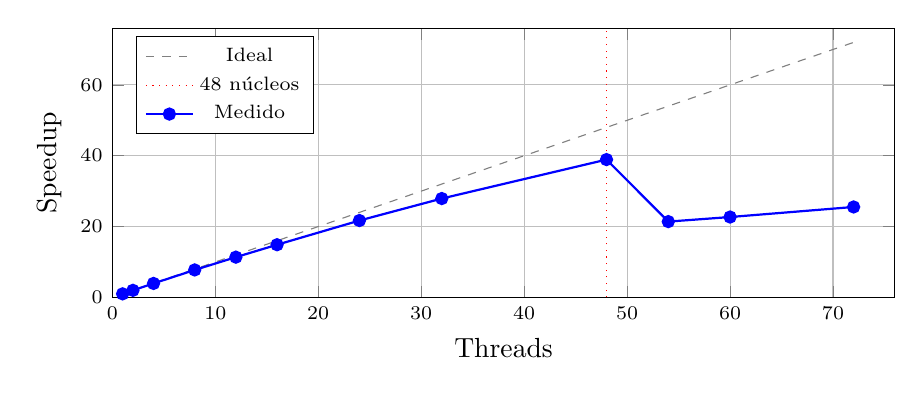
\begin{tikzpicture}
\begin{axis}[width=0.95\columnwidth, height=5cm, xlabel={Threads}, ylabel={Speedup},
  xmin=0, xmax=76, ymin=0, ymax=76, grid=major, legend pos=north west,
  legend style={font=\scriptsize}, tick label style={font=\scriptsize}]
\addplot[dashed, gray] coordinates {(1,1)(72,72)};
\addplot[dotted, red] coordinates {(48,0)(48,76)};
\addplot[mark=*, blue, thick] coordinates {(1,1)(2,1.99)(4,3.94)(8,7.75)(12,11.36)(16,14.87)(24,21.70)(32,27.91)(48,38.91)(54,21.40)(60,22.69)(72,25.53)};
\legend{Ideal, 48 núcleos, Medido}
\end{axis}
\end{tikzpicture}
\caption{Speedup da versão final em função do número de \textit{threads}.}\label{fig:speedup}
\end{figure}

\end{document}
